\documentclass[10pt,a4paper,leqno]{article}         
\usepackage{CJKutf8}                          
\usepackage{inputenc}                         
\usepackage[T1]{fontenc}                      
\usepackage{amsmath,esint}                    
\usepackage{amsfonts}                         
\usepackage{amssymb}                          
\usepackage{xcolor}                           
\usepackage{mathrsfs}                         
\usepackage{makeidx}                          
\usepackage{graphicx}                         
\usepackage{float}                            
\usepackage{textcomp}                         
\usepackage{gensymb}                          
\usepackage{ifpdf}                            
\usepackage{tikz}                             
\usepackage[siunitx]{circuitikz}              
\usetikzlibrary{shapes,arrows,positioning,    
calc,patterns,decorations.pathmorphing,        
decorations.markings}                          
%\usepackage{tgothic}                         
\ifpdf                                        
\usepackage[breaklinks,hidelinks]{hyperref}   
\else                                         
\usepackage{url}                              
\fi                                           
%\newcommand*\VF[1]{\mathbf{#1}}              
%\newcommand*\dif{\mathop{}\!\mathrm{d}}      
\author{CBCO}                           
\title{Mechanical System Diagram in LaTeX Tikz}                             
\begin{document}                              
\maketitle

\noindent \newcommand\CWht[1][2.5]{\tikz[baseline=-#1]{\draw[thick](0,0)     circle[radius=1.5mm];}}
 \par \ \par\noindent \newcommand\CBlk[1][2.5]{\tikz[baseline=-#1]{\draw[thick,    fill=black!](0,0) circle[radius=1.5mm];}}
 \par \ \par\noindent \begin{CJK*}{UTF8}{gbsn}
 \par \ \par\noindent Given the mechanical system free body diagrams as shown in Figure 1, (a) Draw the free body diagram and write the equation for Figure 1 (a) and (b) Draw the free body diagram and write the equation for Figure 1 (b) 
 \par \ \par\noindent \begin{figure}[H]\centering 

 \par \ \par\noindent 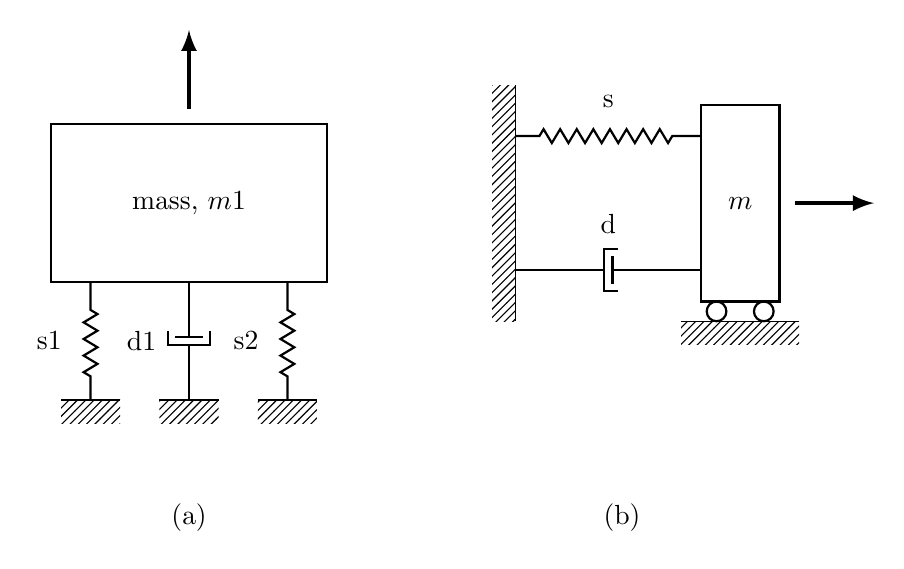
\begin{tikzpicture}[every node/.style={outer sep=0pt,thick}]              
\tikzstyle{spring}=[thick,decorate,decoration={zigzag,pre length=0.3cm,post   
length=0.3cm,segment length=6}]                                                
\tikzstyle{damper}=[thick,decoration={markings,mark connection node=dmp,      
mark=at position 0.5 with                                                      
{                                                                              
\node (dmp) [thick,inner sep=0pt,transform shape,rotate=-90,minimum           
width=15pt,minimum height=3pt,draw=none] {};                                   
\draw [thick] ($(dmp.north east)+(2pt,0)$) -- (dmp.south east) --             
(dmp.south west) -- ($(dmp.north west)+(2pt,0)$);                              
\draw [thick] ($(dmp.north)+(0,-5pt)$) -- ($(dmp.north)+(0,5pt)$);            
}                                                                              
}, decorate]                                                                   
\tikzstyle{ground}=[fill,pattern=north east lines,draw=none,minimum           
width=0.75cm,minimum height=0.3cm]                                             
\node (M) [draw,minimum width=3.5cm,minimum height=2cm] {mass, $m1$};         
\node (ground1) at (M.south) [ground,yshift=-1.5cm,xshift=-1.25cm,            
anchor=north] {};                                                              
\draw (ground1.north west) -- (ground1.north east);                           
\draw [spring] (ground1.north) -- node[left=.25]{s1}($(M.south east)!         
(ground1.north)!(M.south west)$);                                              
\node (ground2) at (M.south) [ground,yshift=-1.5cm,anchor=north] {};          
\draw (ground2.north west) -- (ground2.north east);                           
\draw [damper] (ground2.north) -- node[left=.3]{d1}($(M.south east)!          
(ground2.north)!(M.south west)$);                                              
\node (ground3) at (M.south) [ground,yshift=-1.5cm,xshift=1.25cm,             
anchor=north] {};                                                              
\draw (ground3.north west) -- (ground3.north east);                           
\draw [spring] (ground3.north) -- node[left=.25]{s2}($(M.south east)!         
(ground3.north)!(M.south west)$);                                              
\draw [-latex,ultra thick] (M.north) ++(0,0.2cm) -- +(0,1cm);                  
%                                                                              
\begin{scope}[xshift=7cm]                                                     
\node (M) [draw,minimum width=1cm, minimum height=2.5cm] {$m$};               
\node (ground) [ground,anchor=north,yshift=-0.25cm,minimum width=1.5cm] at    
(M.south) {};                                                                  
\draw (ground.north east) -- (ground.north west);                             
\draw [thick] (M.south west) ++ (0.2cm,-0.125cm) circle (0.125cm)             
(M.south east) ++ (-0.2cm,-0.125cm) circle (0.125cm);                          
\node (wall) [ground, rotate=-90, minimum width=3cm,yshift=-3cm] {};          
\draw (wall.north east) -- (wall.north west);                                 
\draw [spring] (wall.170) -- node[above=.25]{s}($(M.north west)!(wall.170)!   
(M.south west)$);                                                              
\draw [damper] (wall.10) -- node[above=.35]{d}($(M.north west)!(wall.10)!     
(M.south west)$);                                                              
\draw [-latex,ultra thick] (M.east) ++ (0.2cm,0) -- +(1cm,0);                 
\end{scope}                                                                   
%                                                                              
\draw (0cm,-4cm) node{(a)}++(5.5cm,0cm)node{(b)};                             
\end{tikzpicture}
 \par \ \par\noindent \caption{Mechanical System Diagram} \end{figure}
 \par \ \par\noindent The mechanical system in Figure 1 (a) is converted into free body diagram as shown in Figure 2.
 \par \ \par\noindent \begin{figure}[H]\centering 

 \par \ \par\noindent \begin{tikzpicture}[every node/.style={outer sep=0pt,thick}]              
\draw (0cm,0cm) -- (0cm,0cm);                                                 
\node (M) [draw,minimum width=3.5cm,minimum height=2cm] at (5cm,0cm)          
{mass, $m1$};                                                                  
\draw [-latex,ultra thick] (M.north) ++(0cm,0.1cm) -- +(0cm,1cm);             
\draw (5cm,2.4cm) node(){$r(t)
$};                                       
\draw [-latex,ultra thick] (M.south) ++(1cm,-0.1cm) -- +(0cm,-1cm);           
\draw (4cm,-2.5cm) node(){$F_{s1}$};    
\draw [-latex,ultra thick] (M.south) ++(0cm,-0.1cm) -- +(0cm,-1cm);    
\draw (5cm,-2.5cm) node(){$F_{d1}$};    
\draw [-latex,ultra thick] (5cm,-2.75cm)--(5cm,-4cm);        
\draw (5cm,-4.25cm) node(){$F_{mass}$};    
\draw [-latex,ultra thick] (M.south) ++(-1cm,-0.1cm) -- +(0cm,-1cm);    
\draw (6cm,-2.5cm) node(){$F_{s2}$};    
\end{tikzpicture}
 \par \ \par\noindent \caption{Mechanical System Free Body Diagram of Figure 1 (a)} \end{figure}
 \par \ \par\noindent Out of the free diagram in Figure 2, the system equation is generated as follows.
 \par \ \par\begin{equation}
 \begin{minipage}{250pt}
                \begin{flushleft} $\displaystyle F_{d1} + F_{mass} + F_{s1} + F_{s2} = r{\left(t \right)}$  \end{flushleft}
 \end{minipage}
 \end{equation}
\noindent where
 \par \ \par\begin{equation}
 \begin{minipage}{250pt}
                \begin{flushleft} $\displaystyle F_{mass} = m_{1} \frac{d^{2}}{d t^{2}} y{\left(t \right)}$  \end{flushleft}
 \end{minipage}
 \end{equation}
\begin{equation}
 \begin{minipage}{250pt}
                \begin{flushleft} $\displaystyle F_{s1} = K_{1} y{\left(t \right)}$  \end{flushleft}
 \end{minipage}
 \end{equation}
\begin{equation}
 \begin{minipage}{250pt}
                \begin{flushleft} $\displaystyle F_{s2} = K_{2} y{\left(t \right)}$  \end{flushleft}
 \end{minipage}
 \end{equation}
\begin{equation}
 \begin{minipage}{250pt}
                \begin{flushleft} $\displaystyle F_{d1} = b_{1} \frac{d}{d t} y{\left(t \right)}$  \end{flushleft}
 \end{minipage}
 \end{equation}
\noindent Substituting (2), (3), (4), and (5),
 \par \ \par\begin{equation}
 \begin{minipage}{250pt}
                \begin{flushleft} $\displaystyle K_{1} y{\left(t \right)} + K_{2} y{\left(t \right)} + b_{1} \frac{d}{d t} y{\left(t \right)} + m_{1} \frac{d^{2}}{d t^{2}} y{\left(t \right)} = r{\left(t \right)}$  \end{flushleft}
 \end{minipage}
 \end{equation}
\noindent The equation (6) could be arranged for control system block diagram.
 \par \ \par\begin{equation}
 \begin{minipage}{250pt}
                \begin{flushleft} $\displaystyle - b_{1} \frac{d}{d t} y{\left(t \right)} - \left(K_{1} + K_{2}\right) y{\left(t \right)} + r{\left(t \right)} = m_{1} \frac{d^{2}}{d t^{2}} y{\left(t \right)}$  \end{flushleft}
 \end{minipage}
 \end{equation}
\noindent \begin{figure}[H]\centering 

 \par \ \par\noindent \tikzstyle{block} = [draw, fill=white, rectangle,                           
    minimum height=3em, minimum width=6em]                                   
\tikzstyle{sum} = [draw, fill=white, circle, node distance=1cm]             
\tikzstyle{input} = [coordinate]                                            
\tikzstyle{output} = [coordinate]                                           
\tikzstyle{pinstyle} = [pin edge={to-,thin,black}]                          
\begin{tikzpicture}[auto, node distance=2cm,>=latex']                       
\node [input, name=input] {};                                               
\node [sum, right of=input] (sum1) {+};                                     
\node [sum, below of=sum1, node distance = 2 cm] (sum2) {+};                
\node [block, right of=sum1, node distance = 3 cm] (int1)                   
    {$\frac{1}{m1 s}$};                                                     
\node [block, right of=int1, pin={[pinstyle]above:D},                       
            node distance=4cm] (int2) {$\frac{1}{s}$};                      
\node [block, below of=int1] (dfb) {$-b_1$};                                
\draw [->] (int1) -- node[midway](u) {$\frac{dy(t)}{dt}$} (int2);          
\node [output, right of=int2] (output) {};                                  
\node [block, below of=dfb] (fb) {$-(K_1+K_2)$};                            
\draw [draw,->] (input) -- node {$r(t)$} (sum1);                            
\draw [->] (u) |- (dfb.east);                                               
\draw [->] (sum1) -- node {$\frac{m1d^2y(t)}{d^2t}$} (int1);               
\draw [->] (int2) -- node [name=y] {$y(t)$}(output);                        
\draw [->] (y) |- (fb);                                                     
\draw [->] (fb) -| node[below]{$-(K_1+K_2)y(t)$} (sum2)--(sum1) ;           
\draw [->] (dfb) -- node[above]{$-b_1\frac{dy(t)}{dt}$}(sum2);             
\end{tikzpicture} 
 \par \ \par\noindent \caption{Control System Block Diagram} \end{figure}
 \par \ \par\noindent Exercise
 \par \ \par\noindent Use latex for all your drawing. See latex codes above for your referenc.
 \par \ \par\noindent 1. Draw the free body diagram of mechanical system shown in Figure 1 (b).
 \par \ \par\noindent 2. From your free body diagram, derive the equation of the mechanical system.
 \par \ \par\noindent 3. Rearrange your equation for control system block diagram. Generate the control system block diagram.
 \par \ \par\noindent \nocite{2}
 \par \ \par\noindent \nocite{201}
 \par \ \par\noindent \nocite{202}
 \par \ \par\noindent \nocite{301}
 \par \ \par\noindent \nocite{310}
 \par \ \par\noindent \bibliographystyle{plain} 
 \bibliography{ccoLib/ccobib}
 \par \ \par\noindent \end{CJK*}
 \par \ \par\end{document}